\documentclass[border=8pt]{standalone}

\usepackage{tikz}
\usetikzlibrary{arrows.meta,positioning,calc}

% Global compact styling
\tikzset{
  compact/.style={
    every node/.style={font=\small, inner sep=1.2pt},
    line width=0.8pt
  }
}

\begin{document}

% =========================
% 1) Water polarity + hydrogen bond (compact)
% =========================
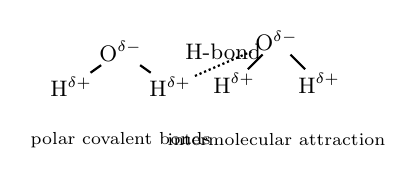
\begin{tikzpicture}[compact, scale=0.9, transform shape]
  \node (O1) at (0,0) {O$^{\delta-}$};
  \node (H1a) at (-0.7,-0.5) {H$^{\delta+}$};
  \node (H1b) at (0.7,-0.5) {H$^{\delta+}$};
  \draw (O1) -- (H1a);
  \draw (O1) -- (H1b);

  \node (O2) at (2.2,0.15) {O$^{\delta-}$};
  \node (H2a) at (1.6,-0.45) {H$^{\delta+}$};
  \node (H2b) at (2.8,-0.45) {H$^{\delta+}$};
  \draw (O2) -- (H2a);
  \draw (O2) -- (H2b);

  \draw[densely dotted, thick] (H1b) -- node[above] {H-bond} (O2);

  \node at (0,-1.25) {\scriptsize polar covalent bonds};
  \node at (2.2,-1.25) {\scriptsize intermolecular attraction};
\end{tikzpicture}

\par\bigskip

% =========================
% 2) Dehydration vs Hydrolysis (COMPACT + VERTICAL)
% =========================
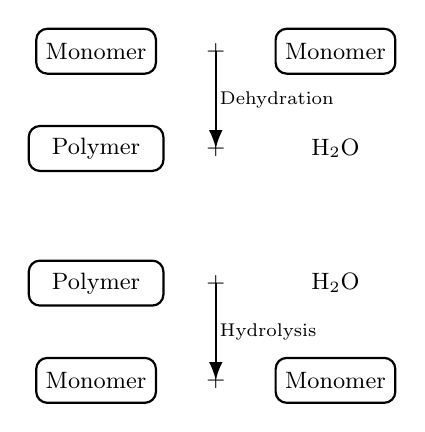
\begin{tikzpicture}[compact, >=Latex, scale=0.95, transform shape]

  % ---------- Dehydration (vertical block) ----------
  \node (dm1) [draw, rounded corners, minimum width=16mm, minimum height=6mm] at (0,0) {Monomer};
  \node (dplus1) at (1.6,0) {+};
  \node (dm2) [draw, rounded corners, minimum width=16mm, minimum height=6mm] at (3.2,0) {Monomer};

  \node (dpoly) [draw, rounded corners, minimum width=18mm, minimum height=6mm] at (0,-1.3) {Polymer};
  \node (dplus2) at (1.6,-1.3) {+};
  \node (dwater) at (3.2,-1.3) {H$_2$O};

  % Arrow down (centered)
  \coordinate (dtop) at ($(dm1)!0.5!(dm2)$);
  \coordinate (dbot) at ($(dpoly)!0.5!(dwater)$);
  \draw[->, thick] (dtop) -- node[right] {\scriptsize Dehydration} (dbot);

  % ---------- Hydrolysis (vertical block, below) ----------
  \node (hpoly) [draw, rounded corners, minimum width=18mm, minimum height=6mm] at (0,-3.1) {Polymer};
  \node (hplus1) at (1.6,-3.1) {+};
  \node (hwater) at (3.2,-3.1) {H$_2$O};

  \node (hm1) [draw, rounded corners, minimum width=16mm, minimum height=6mm] at (0,-4.4) {Monomer};
  \node (hplus2) at (1.6,-4.4) {+};
  \node (hm2) [draw, rounded corners, minimum width=16mm, minimum height=6mm] at (3.2,-4.4) {Monomer};

  \coordinate (htop) at ($(hpoly)!0.5!(hwater)$);
  \coordinate (hbot) at ($(hm1)!0.5!(hm2)$);
  \draw[->, thick] (htop) -- node[right] {\scriptsize Hydrolysis} (hbot);

\end{tikzpicture}

\par\bigskip

% =========================
% 3) General amino acid structure (compact)
% =========================
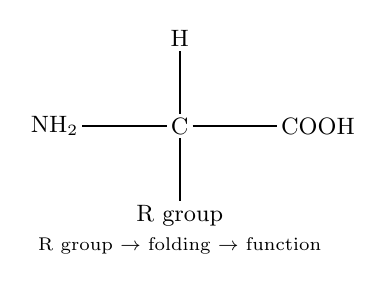
\begin{tikzpicture}[compact, scale=0.95, transform shape]
  \node (C) at (0,0) {C};
  \draw (C) -- (0,1.0) node[above] {H};
  \draw (C) -- (-1.3,0) node[left] {NH$_2$};
  \draw (C) -- (1.3,0) node[right] {COOH};
  \draw (C) -- (0,-1.0) node[below] {R group};

  \node at (0,-1.6) {\scriptsize R group $\rightarrow$ folding $\rightarrow$ function};
\end{tikzpicture}

\par\bigskip

% =========================
% 4) Linear vs branched polysaccharide (compact)
% =========================
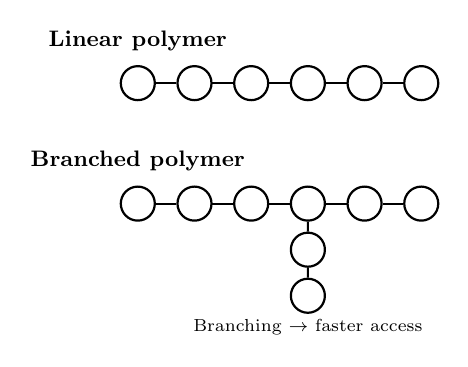
\begin{tikzpicture}[compact, scale=0.9, transform shape]
  % Linear
  \node[font=\small\bfseries] at (0,1.6) {Linear polymer};
  \foreach \i in {0,...,5} {
    \node[draw, circle, minimum size=4.8mm] (L\i) at (\i*0.8,1.0) {};
    \ifnum\i>0
      \draw (L\the\numexpr\i-1\relax) -- (L\i);
    \fi
  }

  % Branched
  \node[font=\small\bfseries] at (0,-0.1) {Branched polymer};
  \foreach \i in {0,...,5} {
    \node[draw, circle, minimum size=4.8mm] (B\i) at (\i*0.8,-0.7) {};
    \ifnum\i>0
      \draw (B\the\numexpr\i-1\relax) -- (B\i);
    \fi
  }
  \node[draw, circle, minimum size=4.8mm] (Br1) at (2.4,-1.35) {};
  \node[draw, circle, minimum size=4.8mm] (Br2) at (2.4,-2.0) {};
  \draw (B3) -- (Br1) -- (Br2);

  \node at (2.4,-2.45) {\scriptsize Branching $\rightarrow$ faster access};
\end{tikzpicture}

\end{document}
